\documentclass[11pt]{article}
\usepackage{pdfpages}
\usepackage{blindtext}
\usepackage{relsize}
\usepackage{tocloft}
%\usepackage{titling}
%\predate{}
%\postdate{}
\author{https://slds-lmu.github.io/i2ml/}
\title{Introduction to Machine Learning\\[0.2em]\smaller{}All exercises}
\date{Winterterm 2022/2023} % clear date
\renewcommand{\cftsecleader}{\cftdotfill{\cftdotsep}}
\newcommand{\fakesection}[1]{%
  \par\refstepcounter{section}% Increase section counter
  \sectionmark{#1}% Add section mark (header)
  \addcontentsline{toc}{section}{\protect\numberline{\thesection}#1}% Add section to ToC
  % Add more content here, if needed.
}

\begin{document}
\maketitle
\tableofcontents
\clearpage


% General remark: hyperlinks in included pdfs are not clickable anymore in the combined pdf

% Include tuning lecture slides
\fakesection{Exercise 1 - ML Basics}
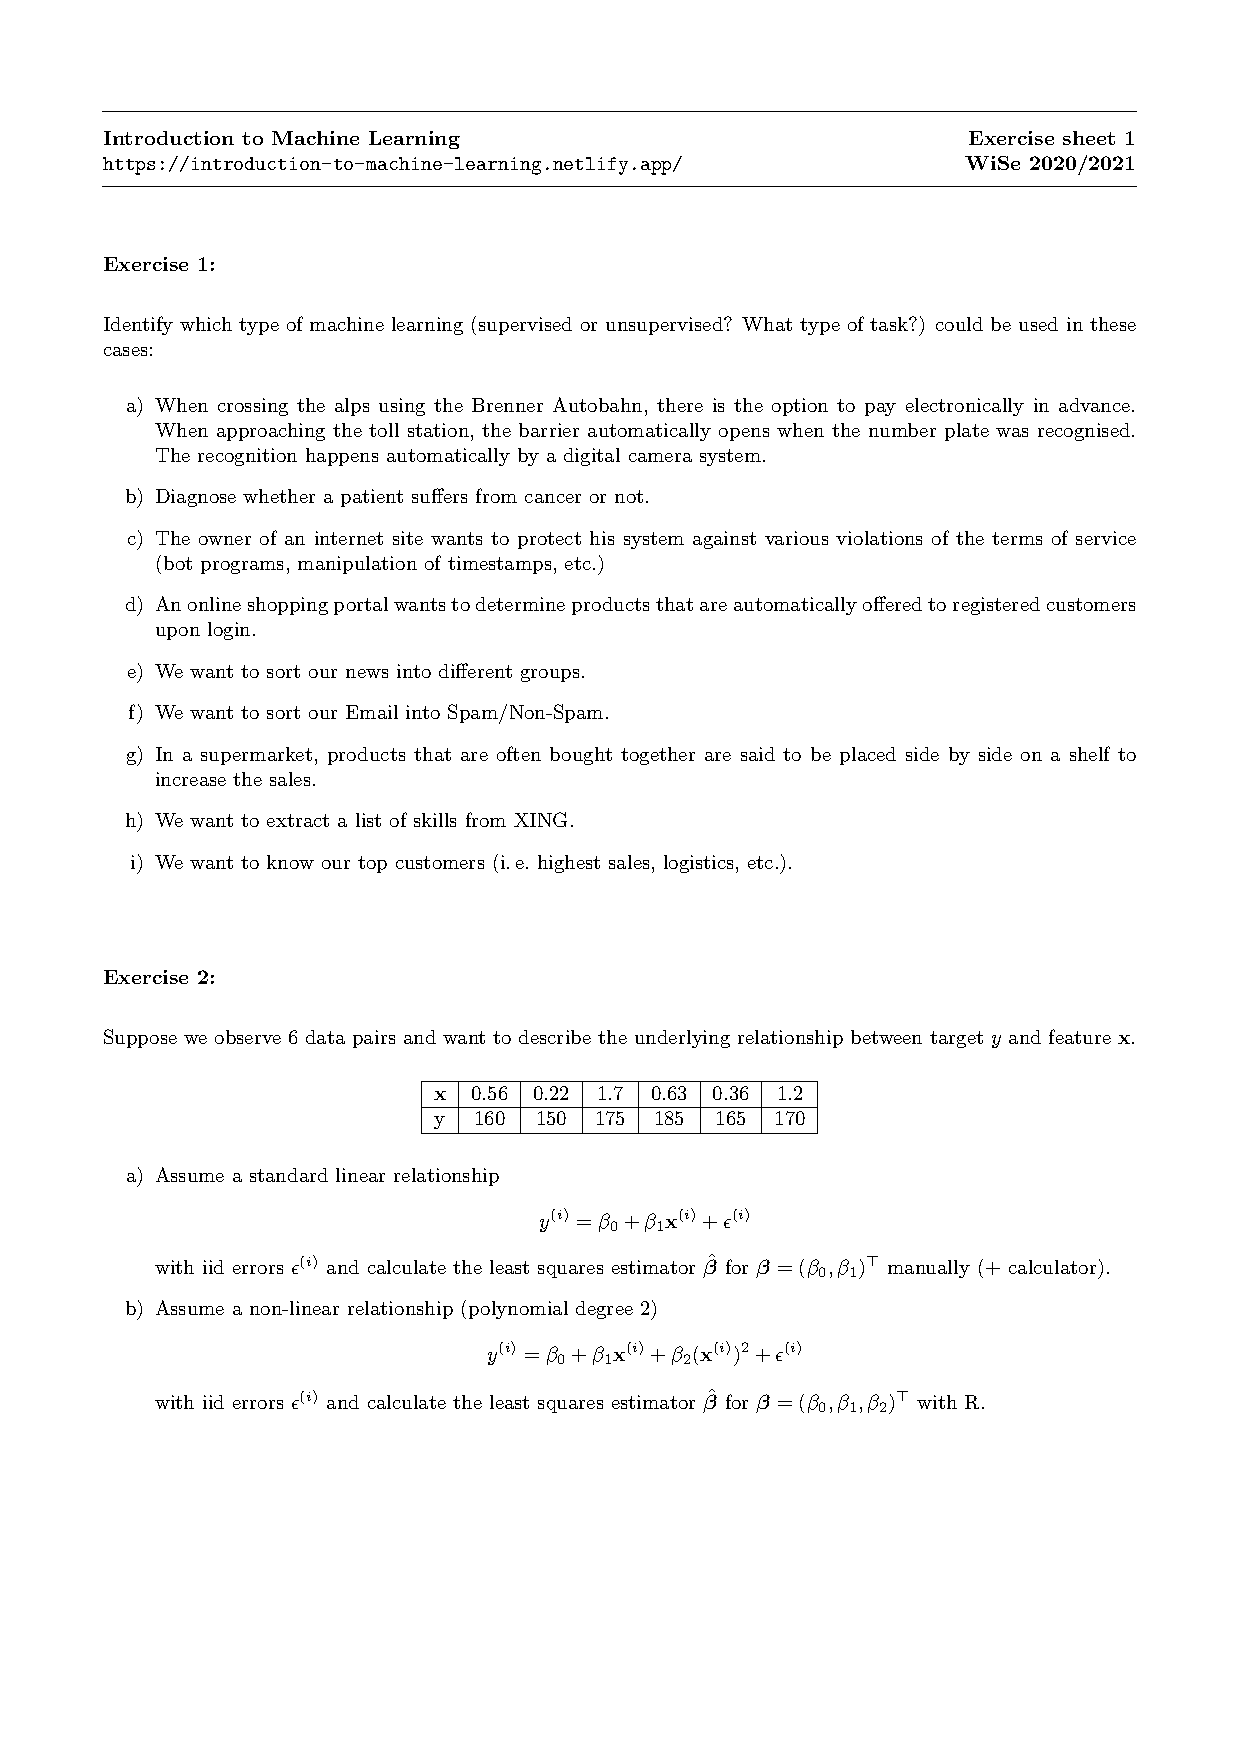
\includepdf[pages=-, pagecommand=\label{ml_basics}]{../exercises-pdf/ex_ml-basics.pdf}

\fakesection{Exercise 2 - Supervised Regression}
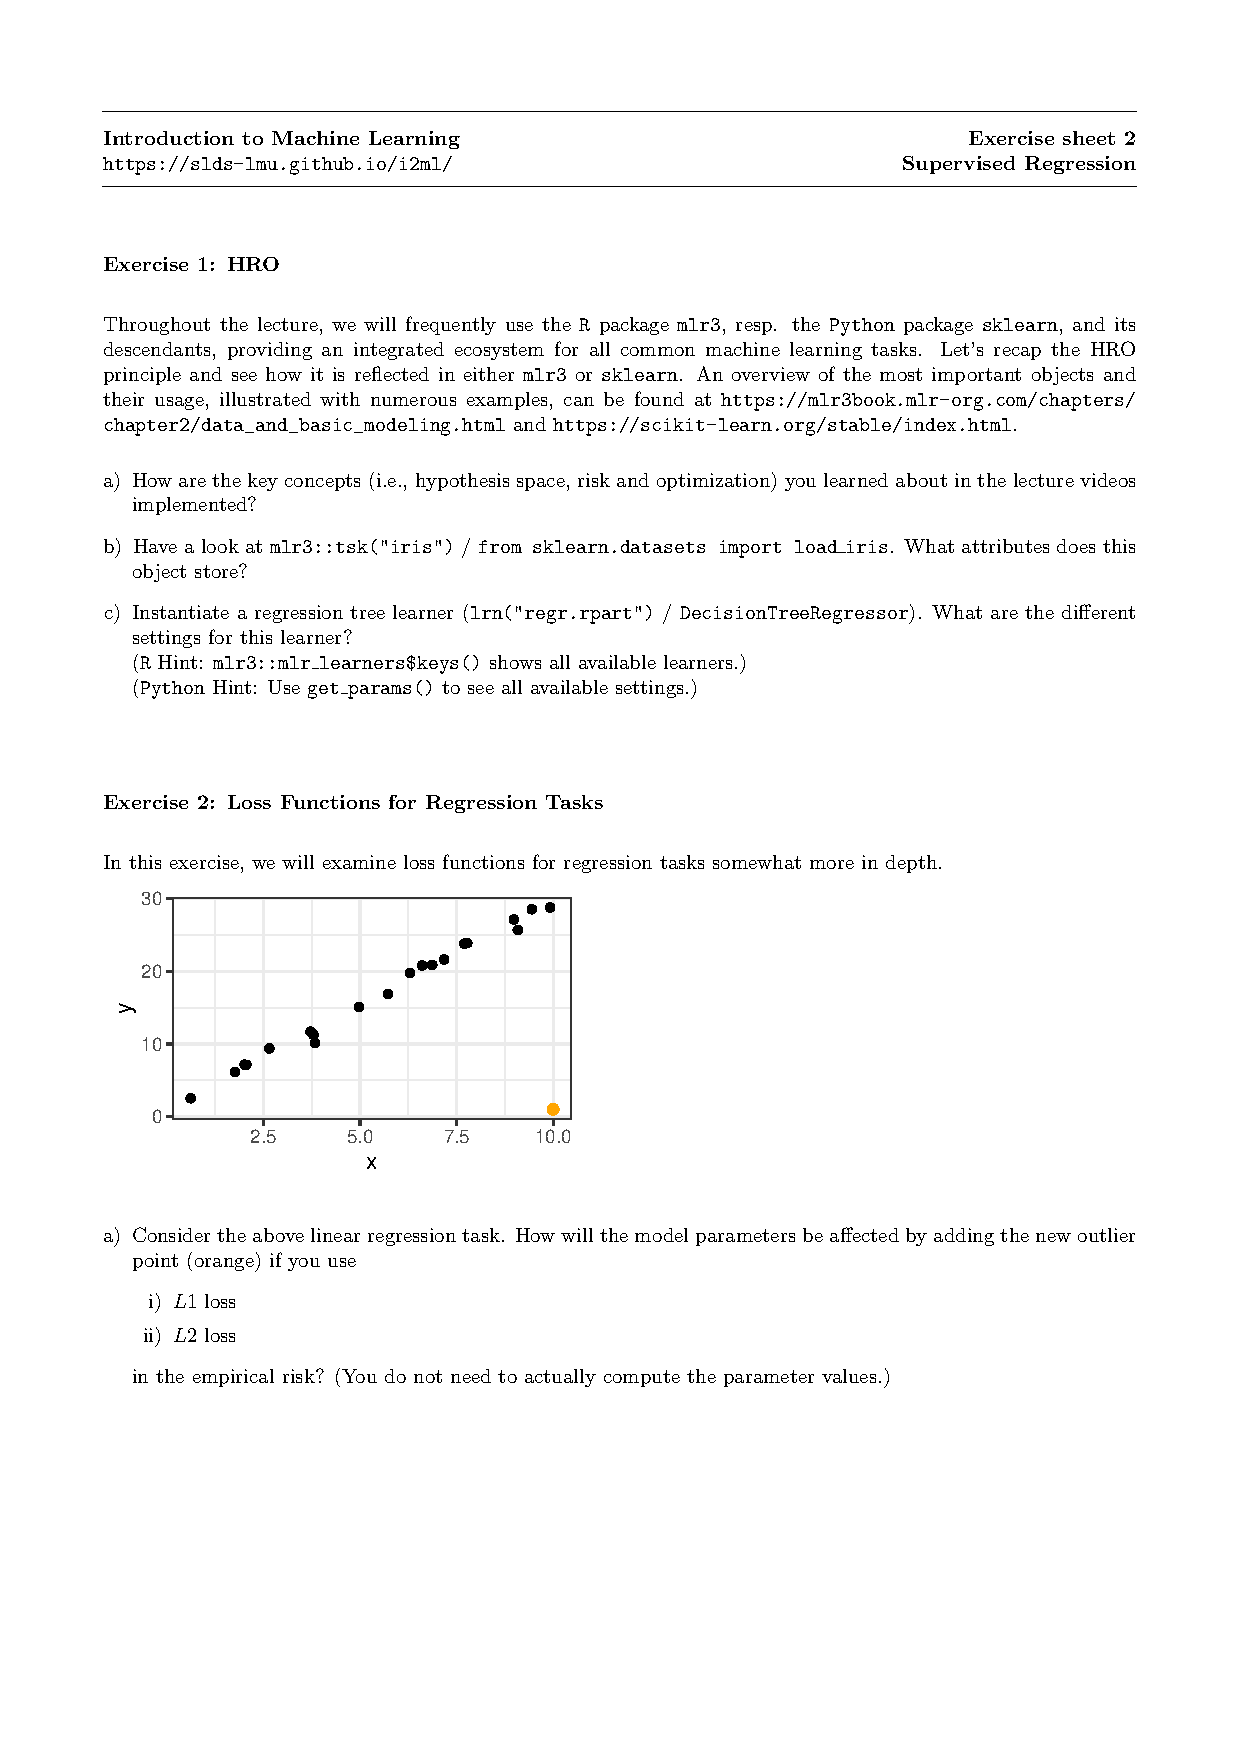
\includepdf[pages=-]{../exercises-pdf/ex_regression.pdf}

\fakesection{Exercise 3 - Supervised Classification 1}
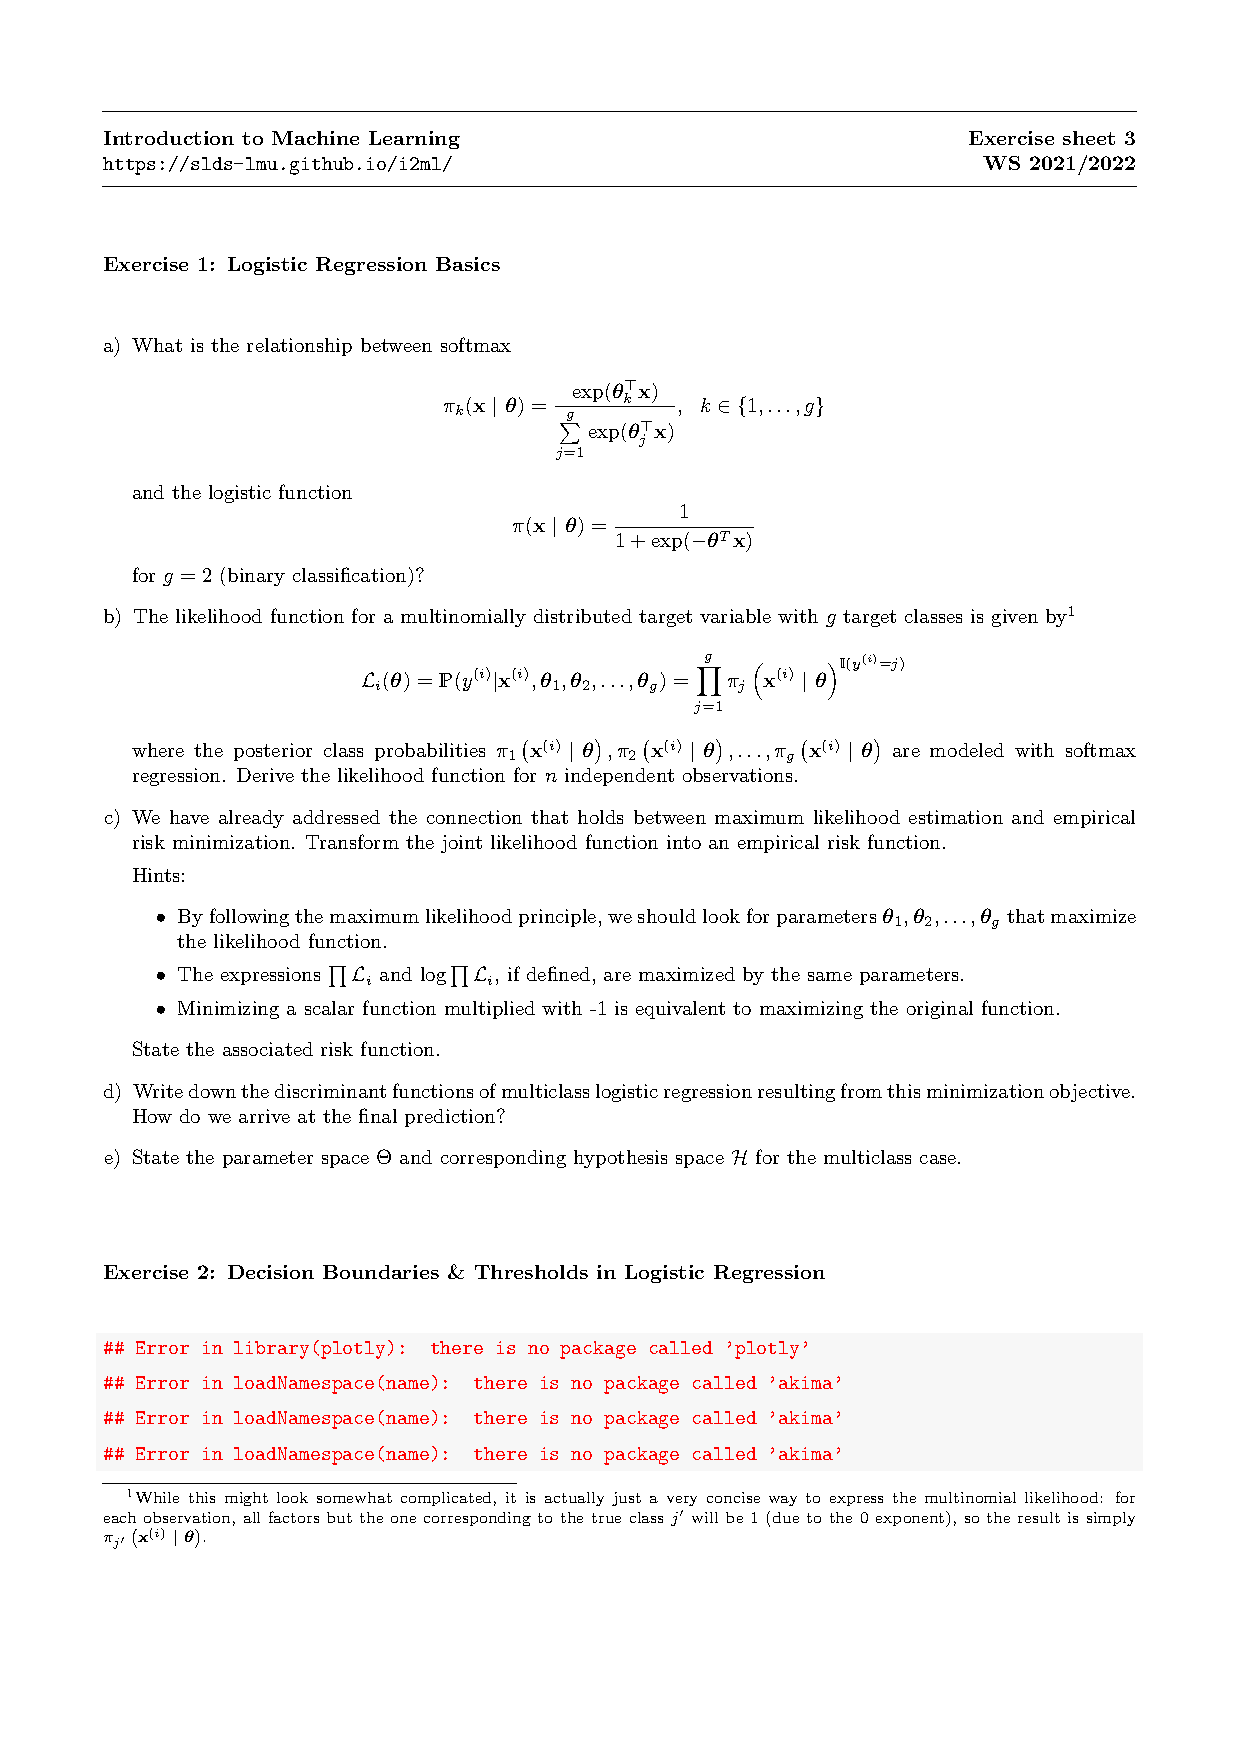
\includepdf[pages=-]{../exercises-pdf/ex_classification_1.pdf}

\fakesection{Exercise 4 - Supervised Classification 2}
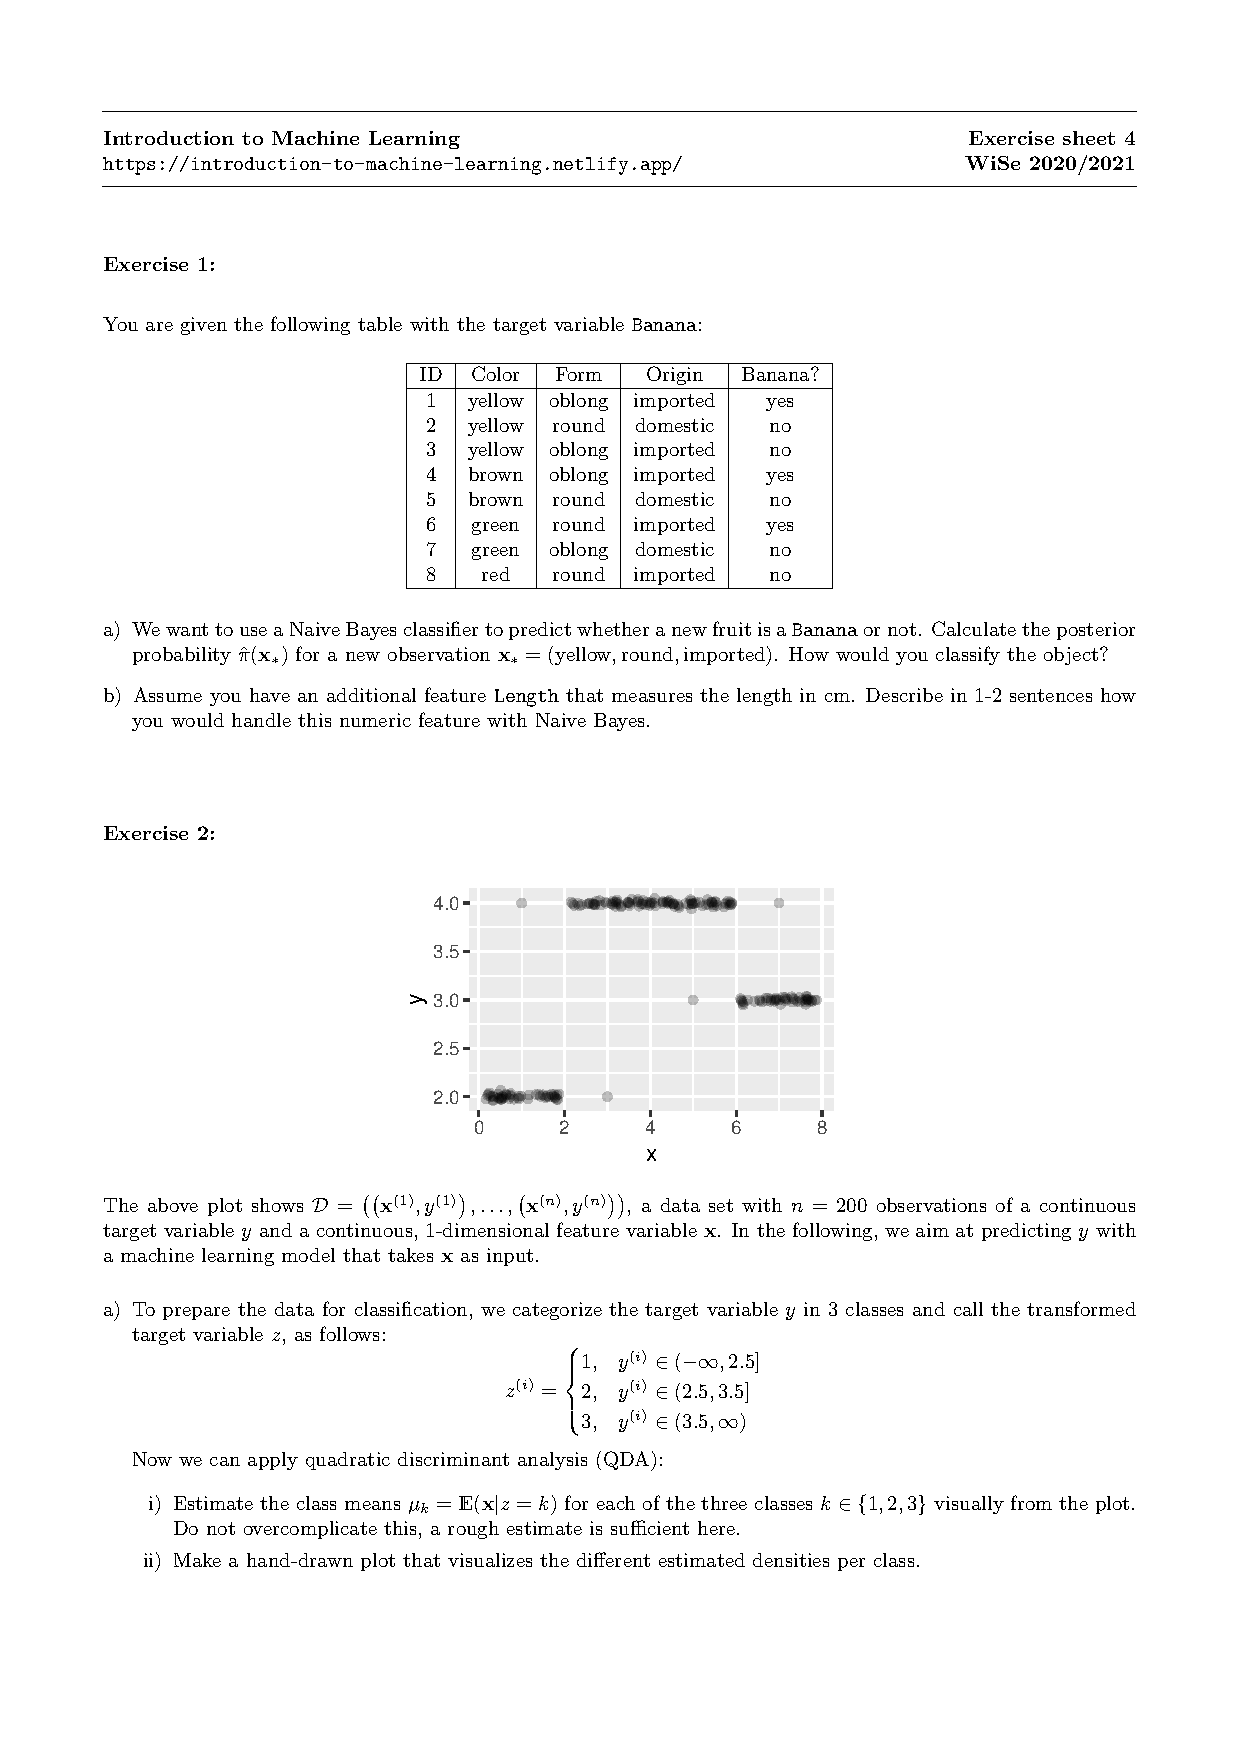
\includepdf[pages=-]{../exercises-pdf/ex_classification_2.pdf}

\fakesection{Exercise 5 - Performance Evaluation 1}
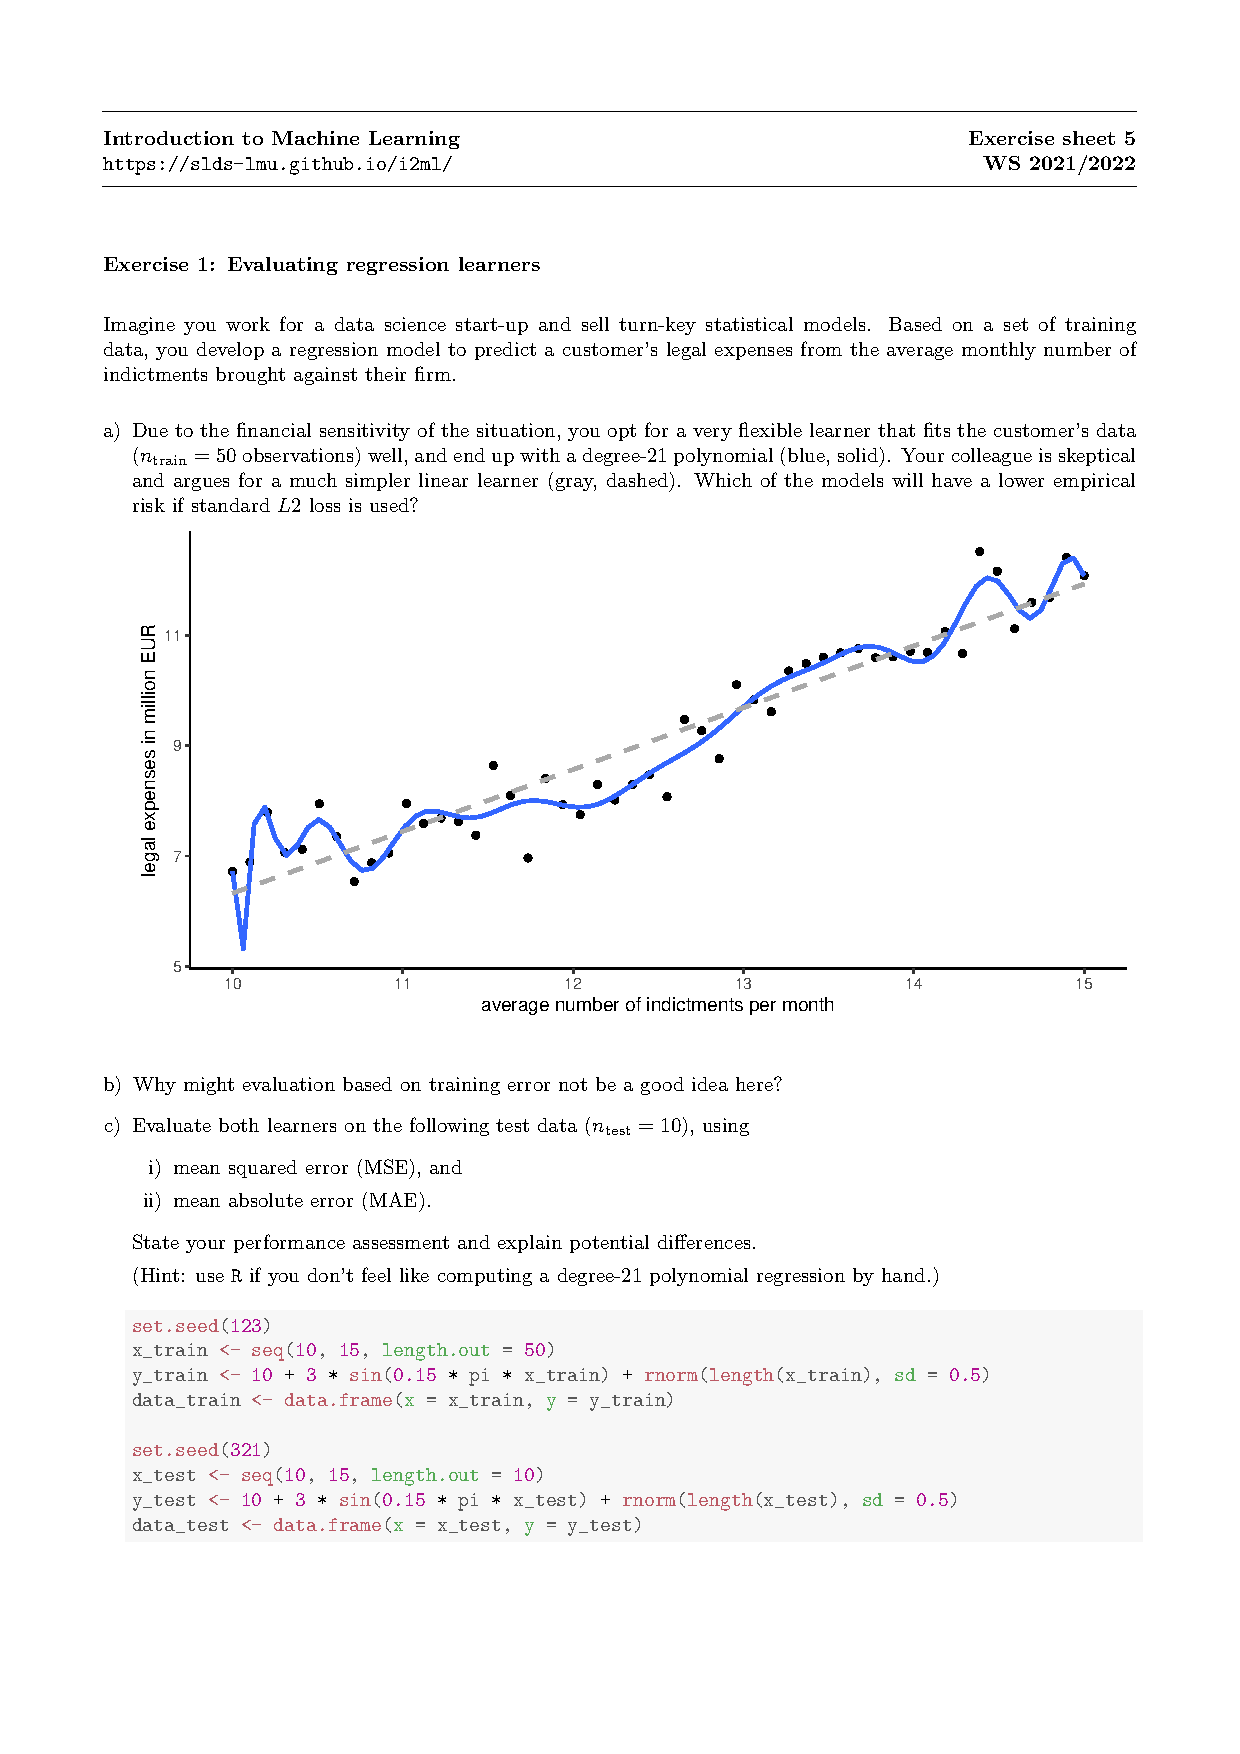
\includepdf[pages=-]{../exercises-pdf/ex_eval_1.pdf}
\fakesection{Exercise 6 - Performance Evaluation 2}
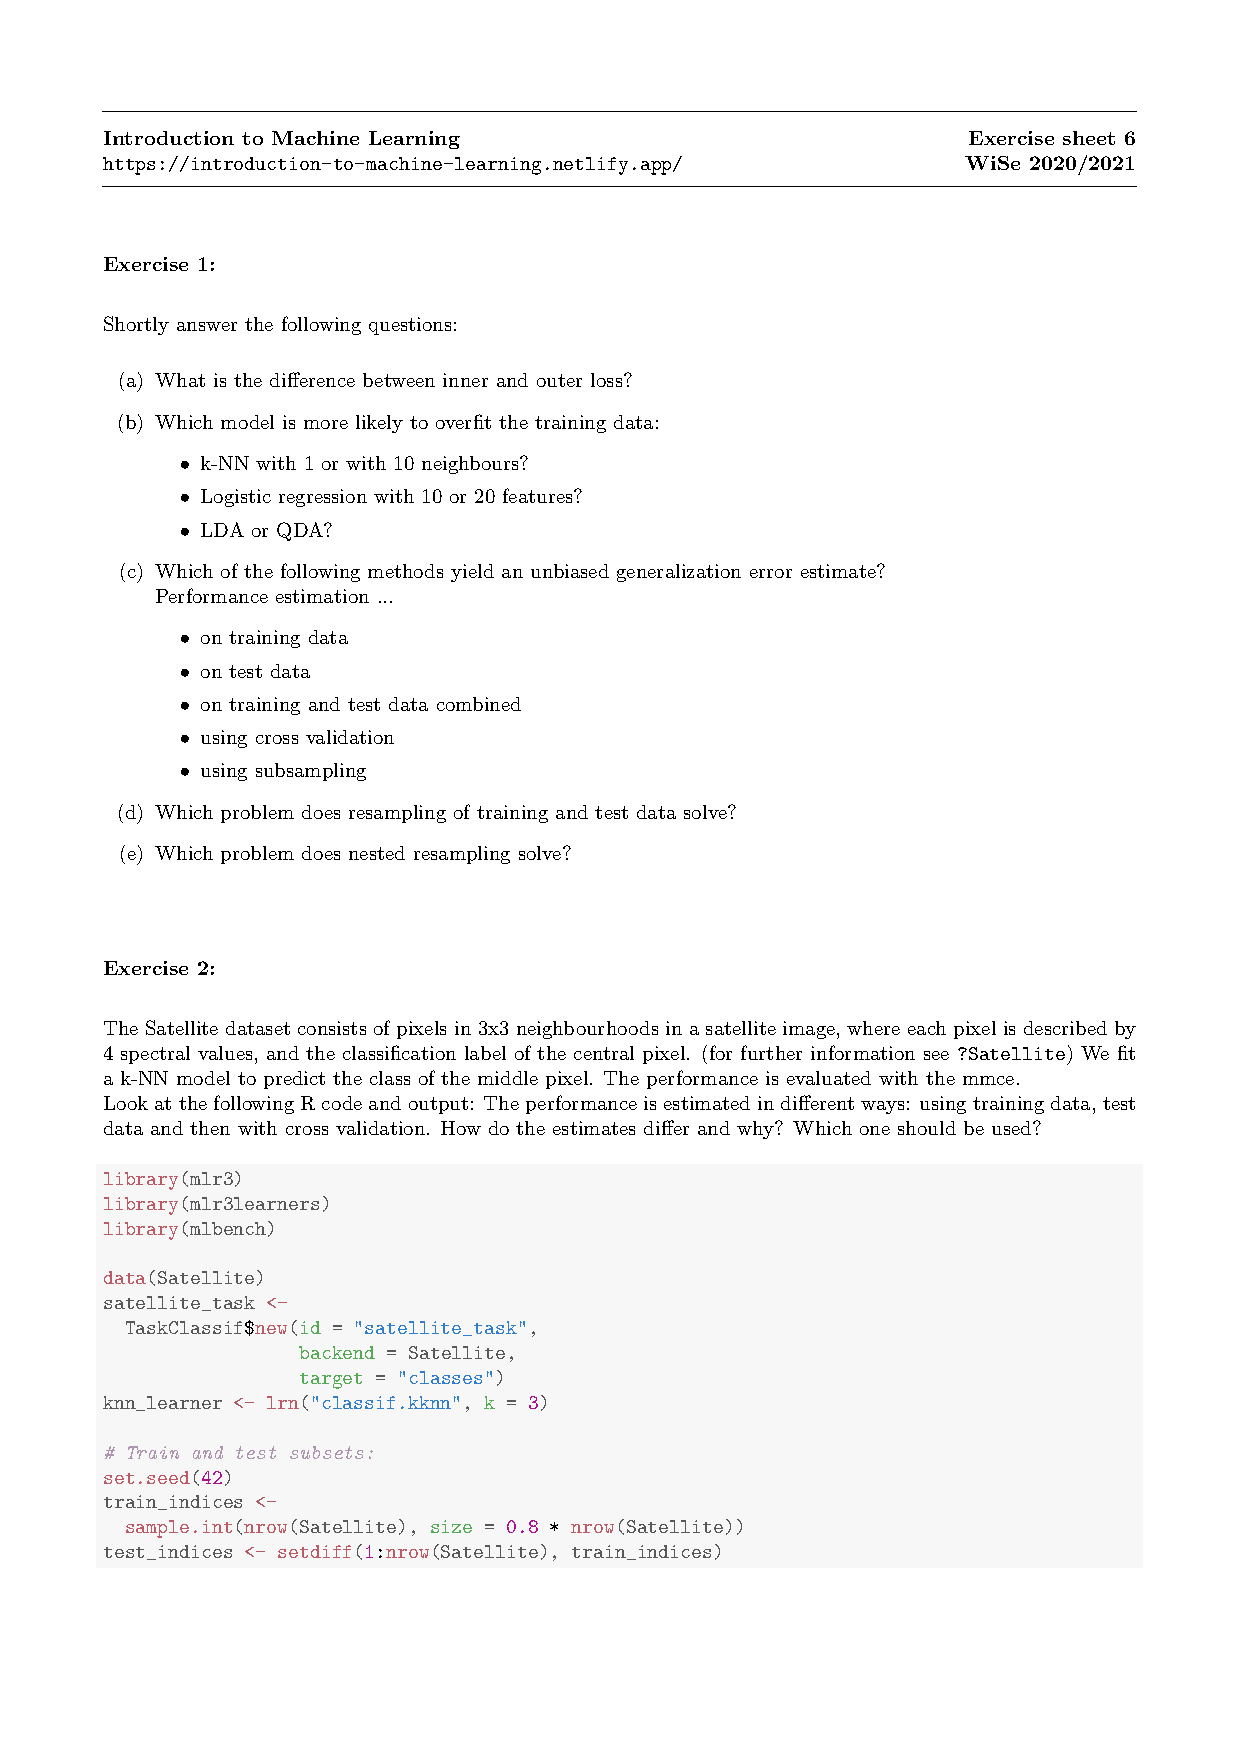
\includepdf[pages=-]{../exercises-pdf/ex_eval_2.pdf}
\fakesection{Exercise 7 - Performance Evaluation 3}
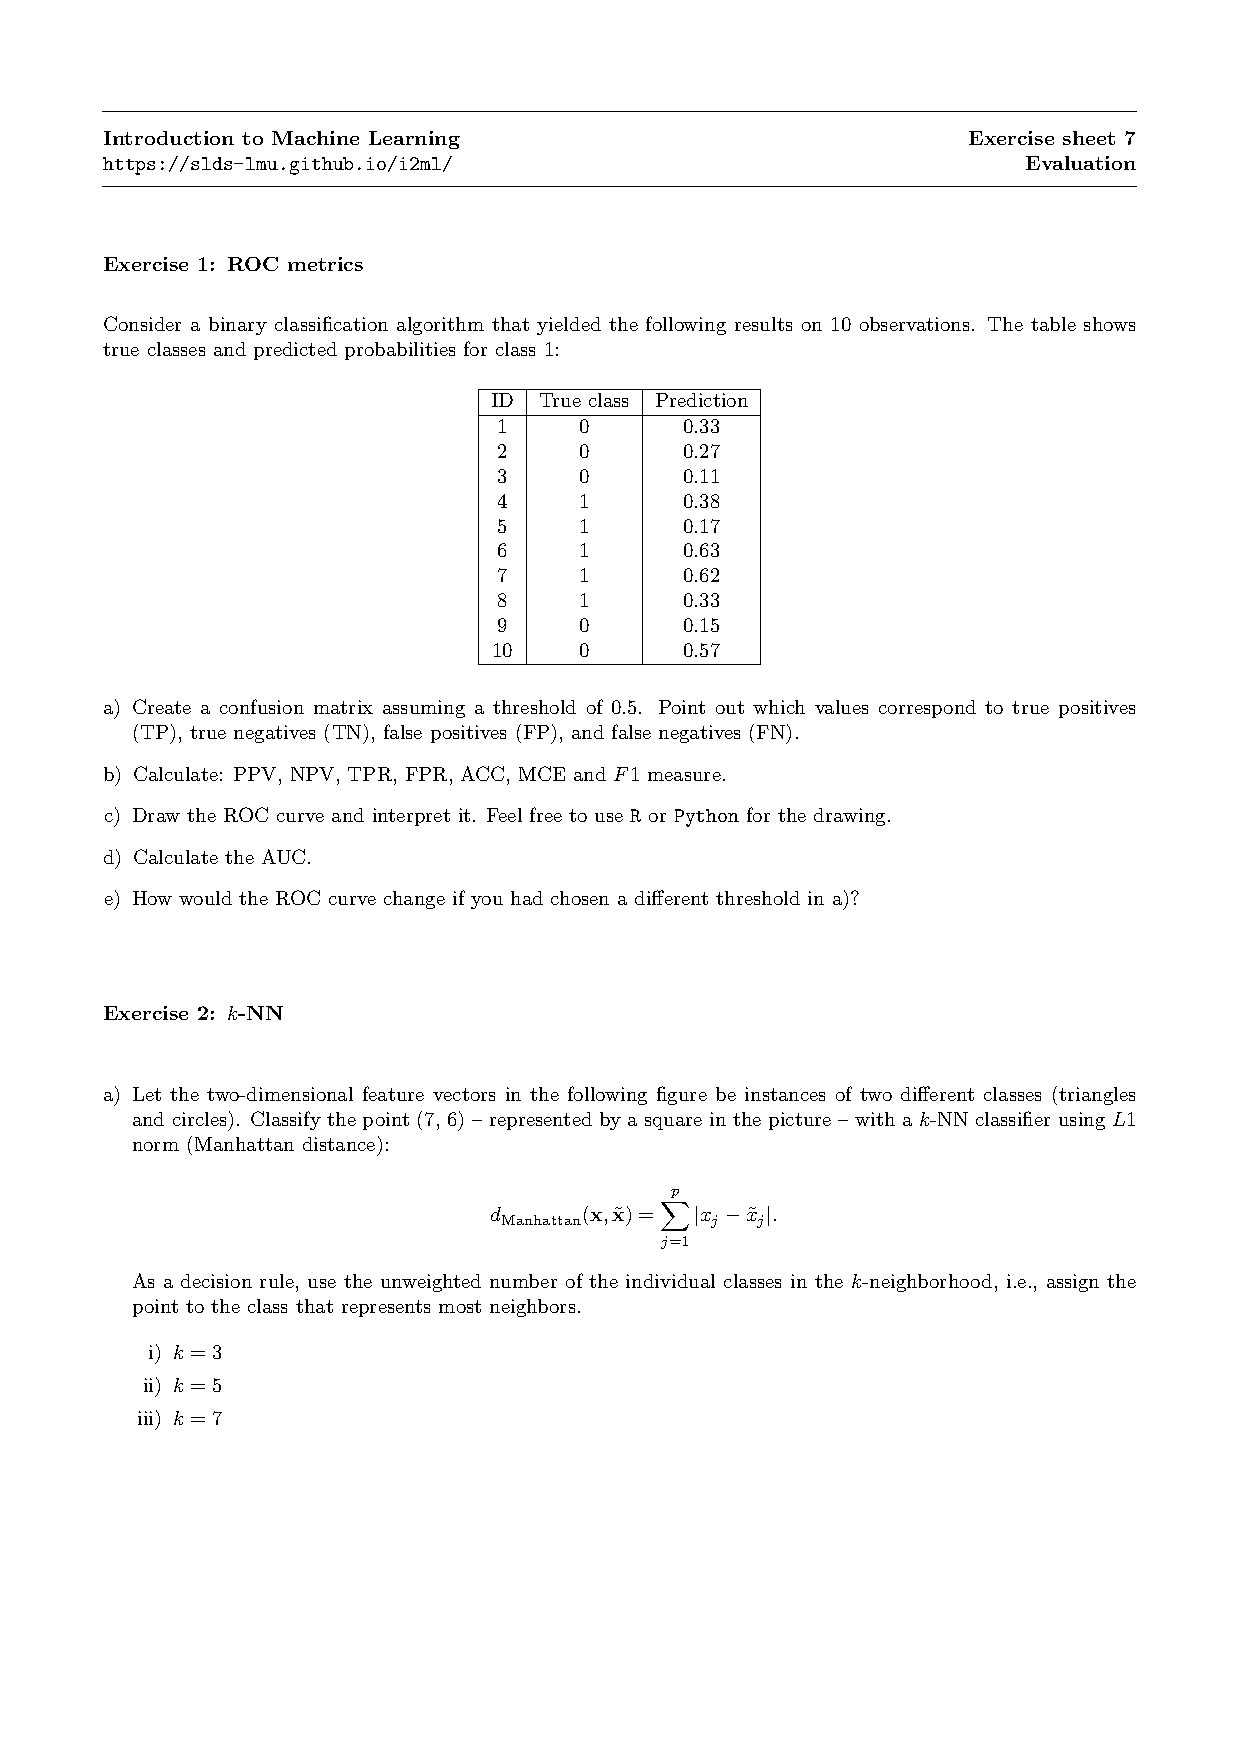
\includepdf[pages=-]{../exercises-pdf/ex_eval_3.pdf}


\fakesection{Exercise 8 - Classification and Regression Trees (CART)}
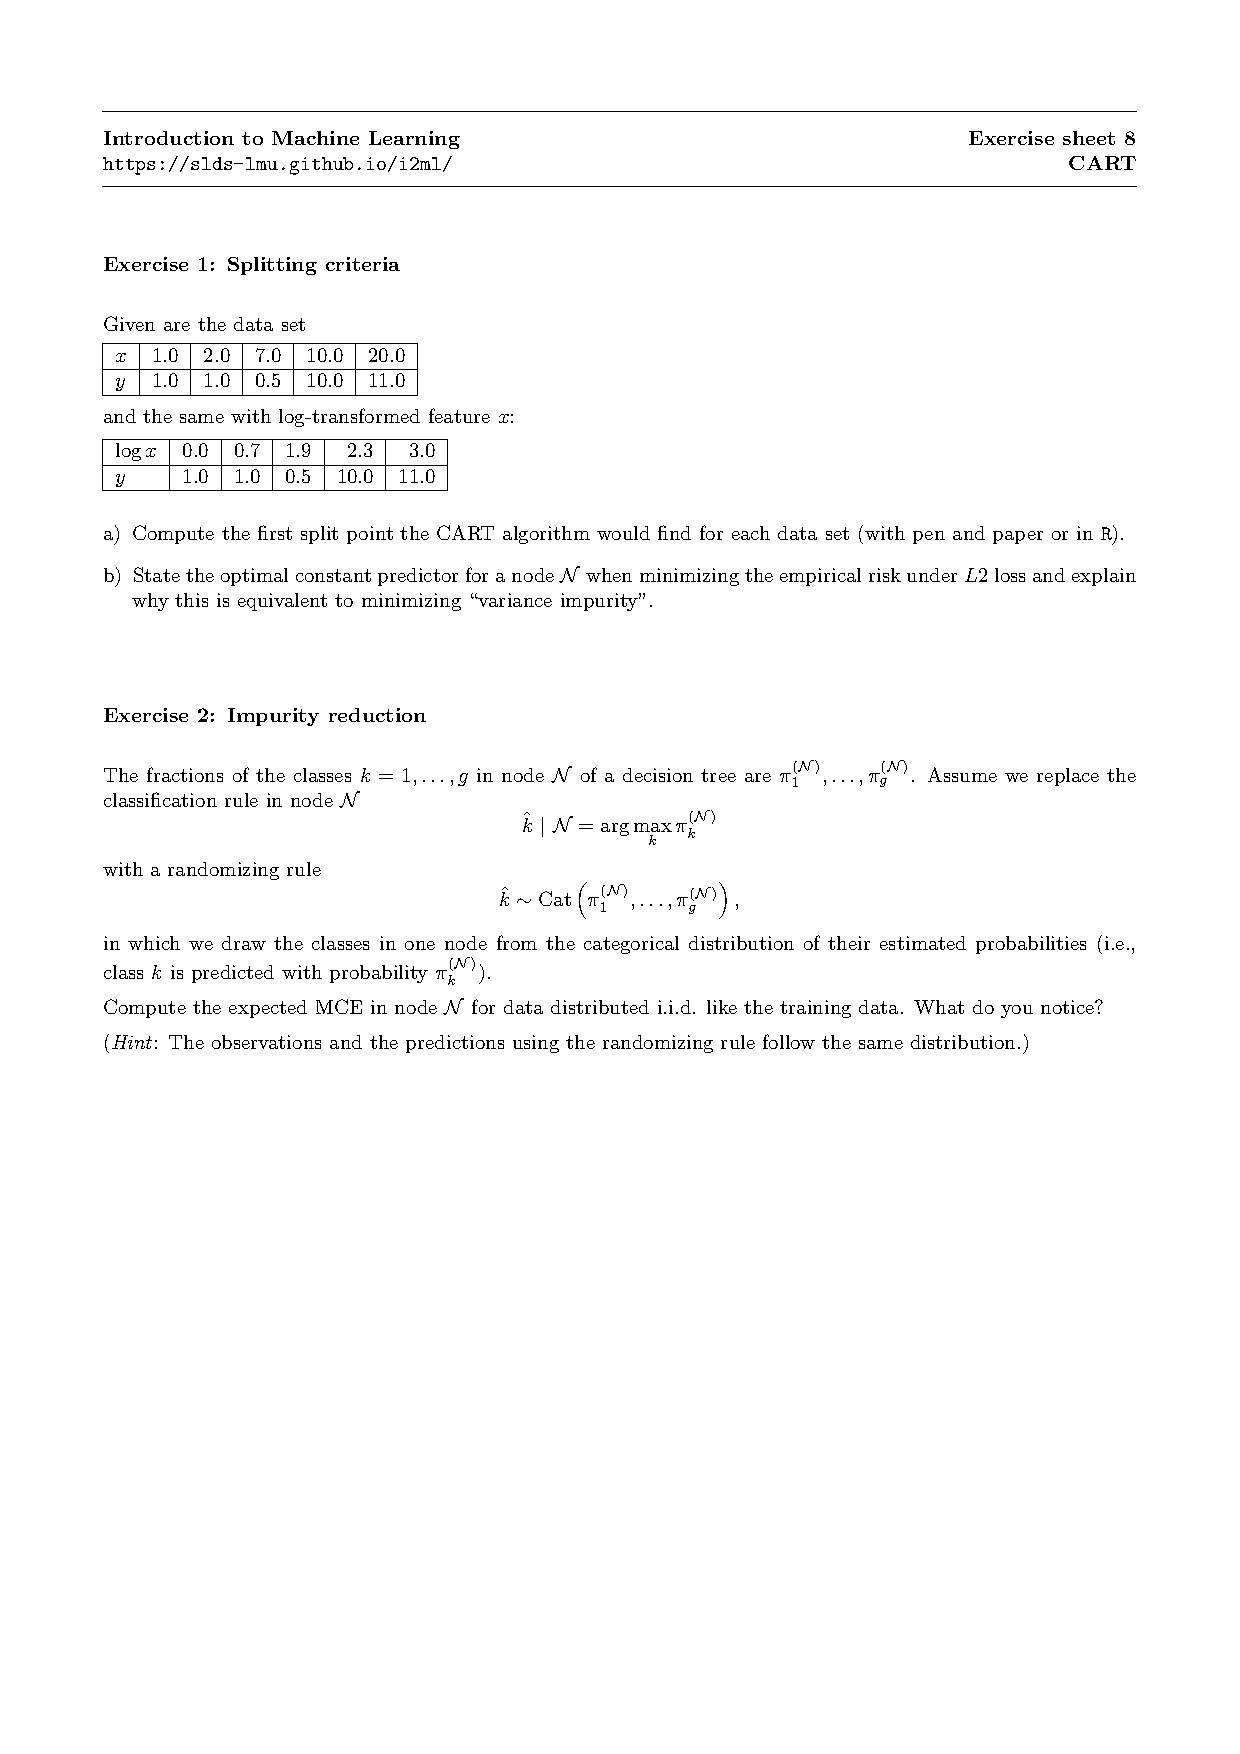
\includepdf[pages=-]{../exercises-pdf/ex_trees.pdf}

\fakesection{Exercise 9 - Random Forests}
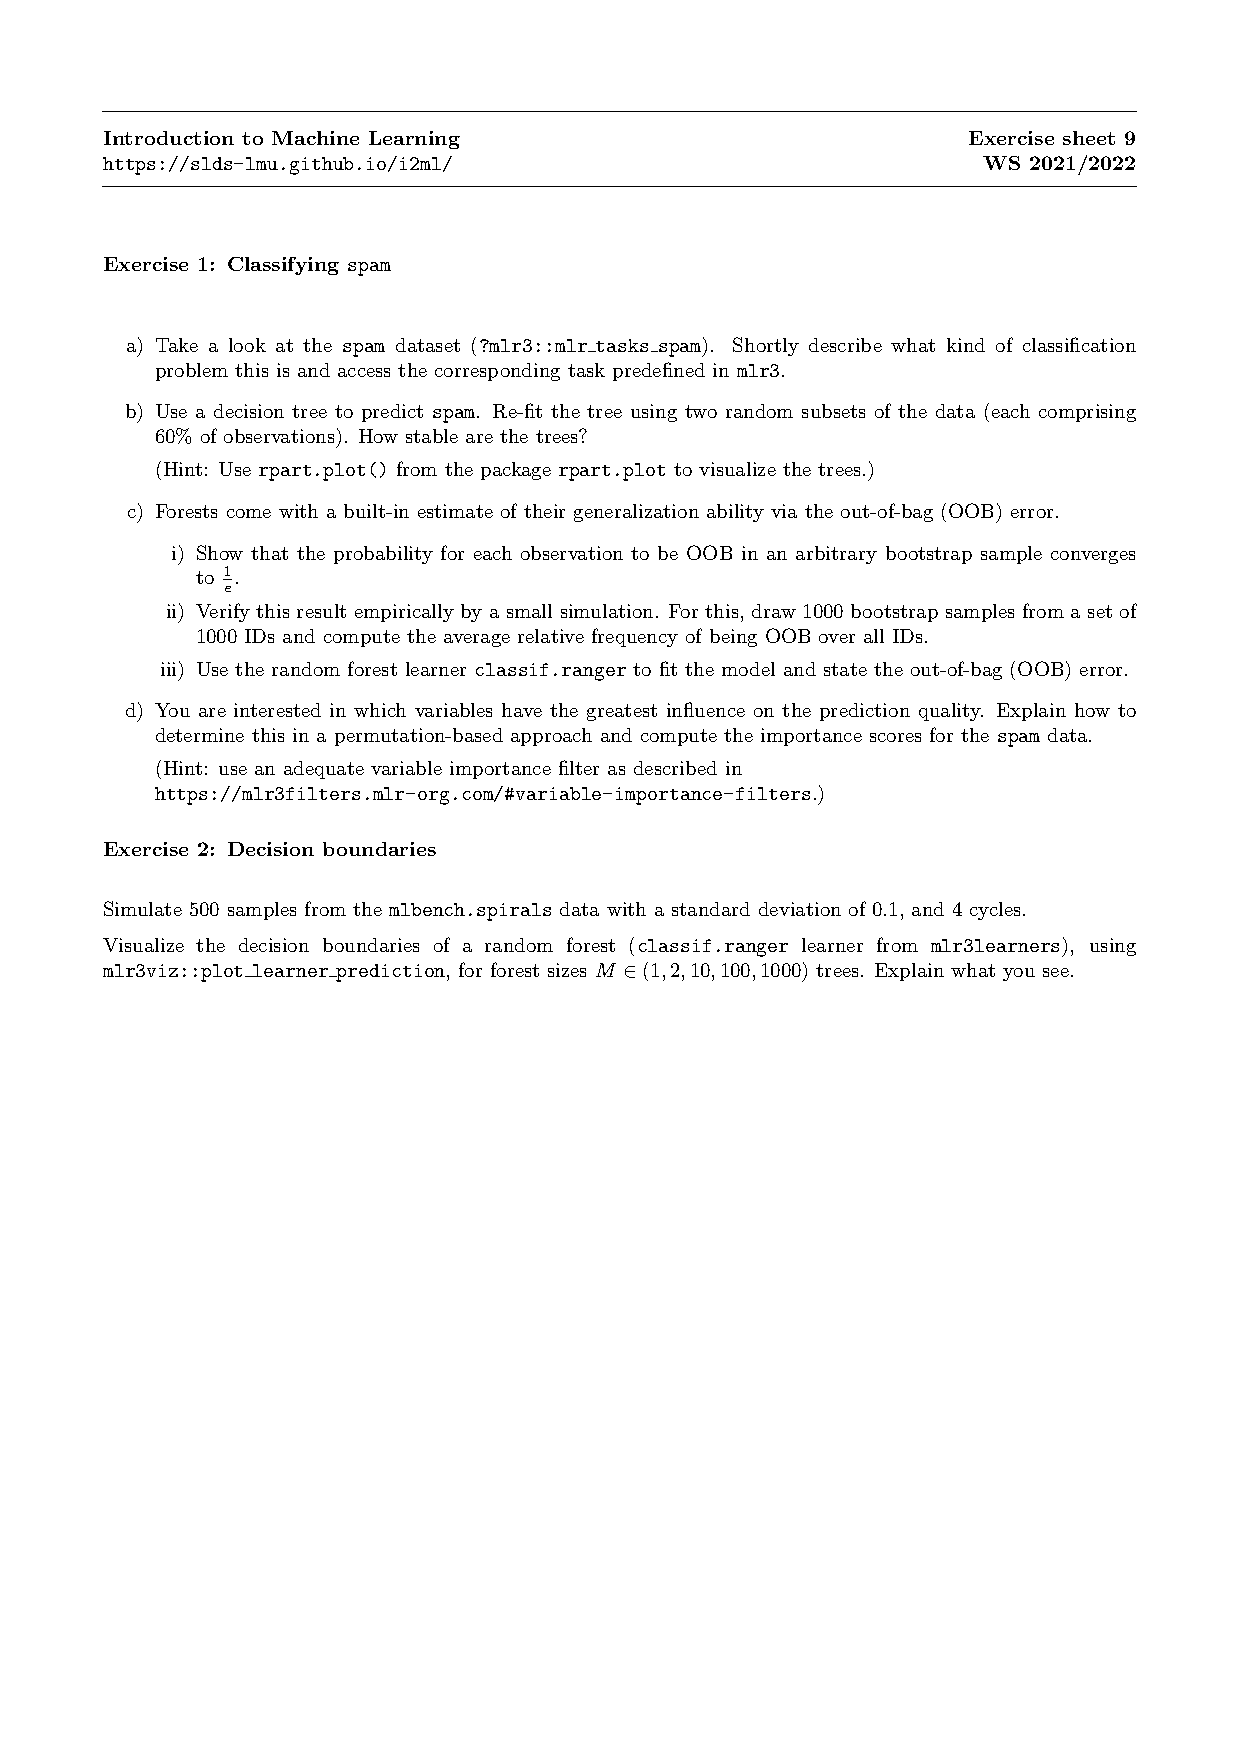
\includepdf[pages=-]{../exercises-pdf/ex_forests.pdf}

%\fakesection{Tuning}
%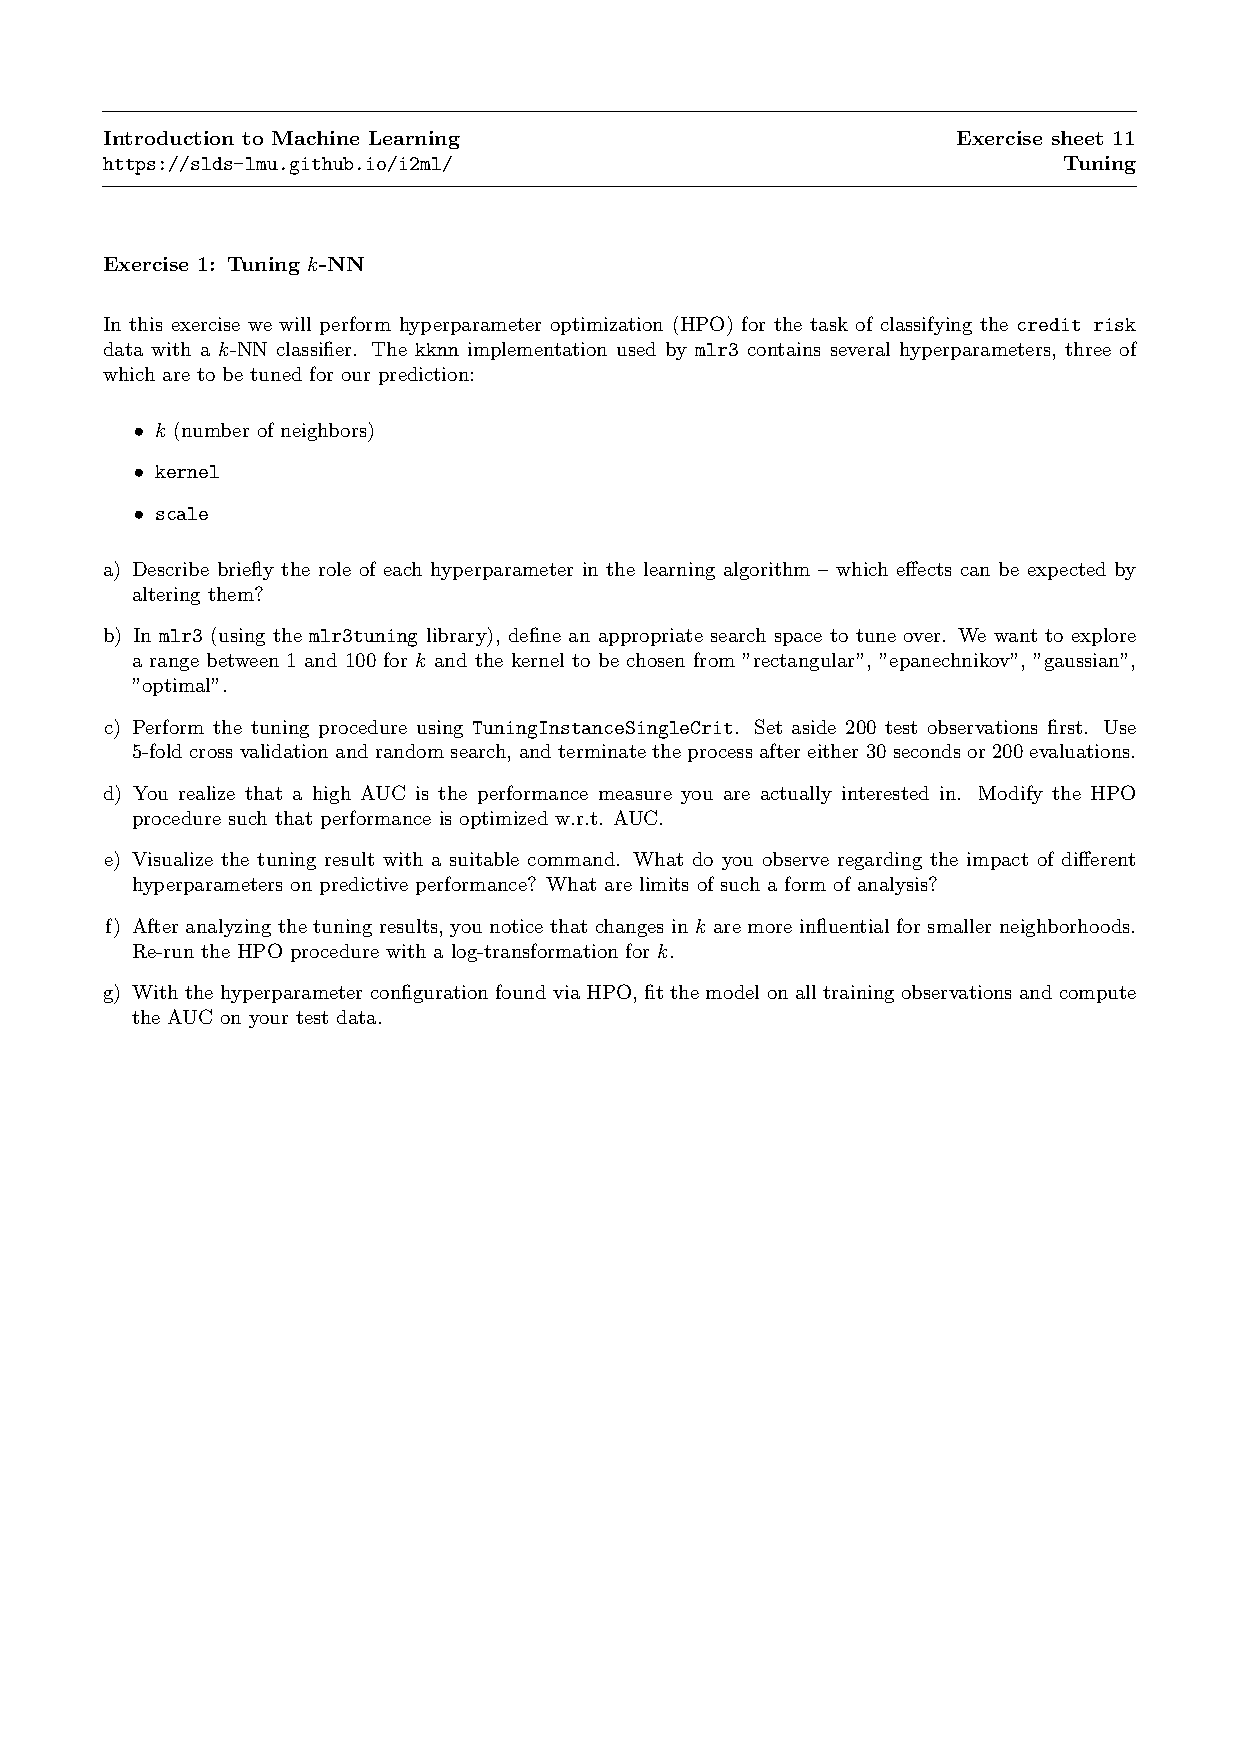
\includepdf[pages=-]{../exercises-pdf/ex_tuning.pdf}

\fakesection{Exercise 10 - Tuning, Nested Resampling and mlr3}
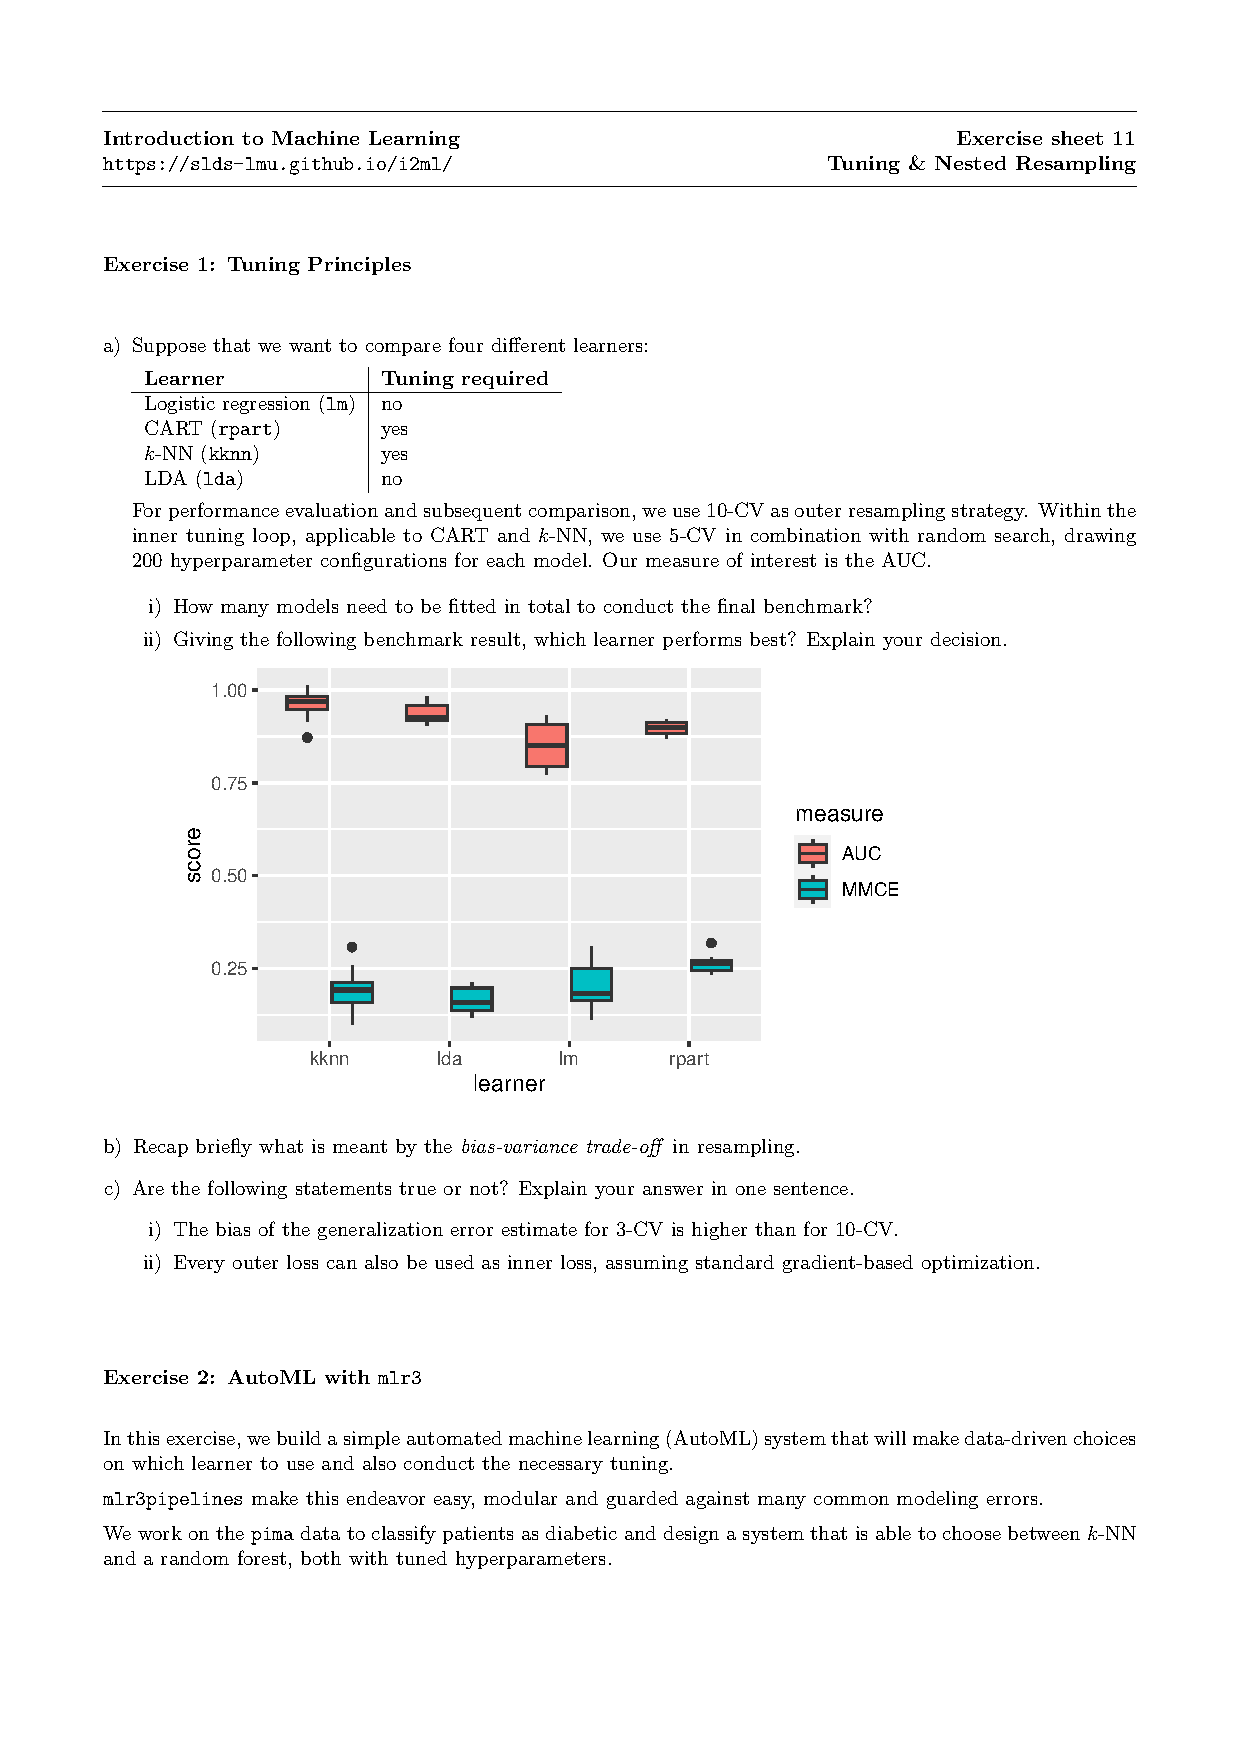
\includepdf[pages=-]{../exercises-pdf/ex_tuning_resampling.pdf}


\end{document}
